\testCom
{%Номер задачи
	3.152
}
{%Условие
	условие
}
{%Дано
	дано
}
{%Найти
	найти
}
{%Решение
	%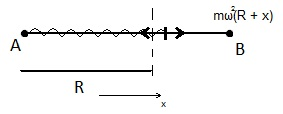
\includegraphics[height=30mm]{3_33.jpg}\\
	Очевидно (3.150), что $U _L ~ I_m ~ \frac{1}{\abs{Z}}$\\
	$\abs{Z} \rightarrow min \Rightarrow \frac{1}{\omega C} - L \omega = 0 \Rightarrow C = \frac{1}{\omega^2 L}$\\
	$U_L = I_m \sqrt{R^2 + \omega^2 L^2} = \frac{U_m}{R} \sqrt{R^2 + (\omega L)^2}= U_m  \sqrt{1 + (\frac{\omega L}{R})^2}$\\
	$U_C = I_m \frac{1}{\omega C} = \frac{U_m}{R} \cdot L \omega = U_m \frac{L \omega}{R}$\\
}

